\section{Factorial}

\subsection{Objective}

To write a program to calculate the factorial of a number.

\subsection{Implementation}

The factorial of a number $n$ is calculated using the following formula:

\begin{equation}
    n! = n \times (n-1) \times (n-2) \times \cdots \times 1
\end{equation}

\subsubsection{Assembly code}

\asmcode{./code/8086/fact.asm}

\pagebreak
\subsection{Output}

\subsubsection{Discussion}

The factorial of 7:

\begin{equation}
    7! = 5040_{10} = 13B0_{16}
\end{equation}

Which can be seen in Figure \ref{fig:fact} at the start of the DS segment.

\begin{figure}[ht]
    \centering
    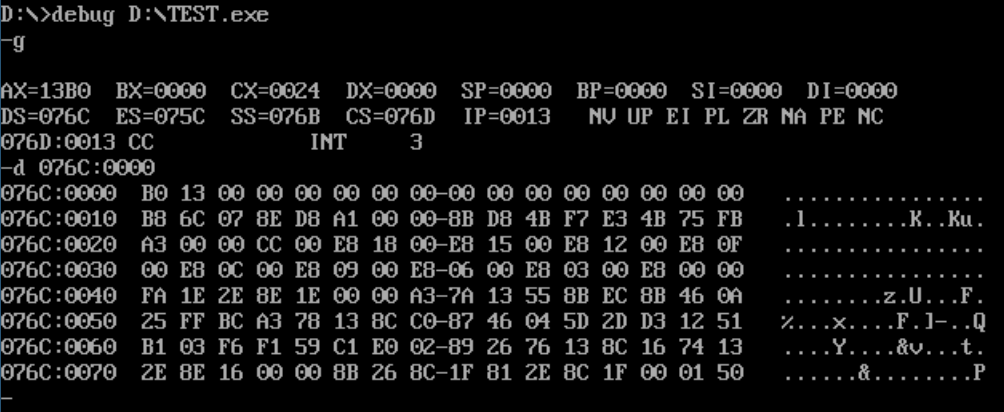
\includegraphics[width=0.8\textwidth]{./res/practicals/fact.png}
    \caption{Factorial program}
    \label{fig:fact}
\end{figure}

